\chapter{Results}\label{chapter:results}\textcolor{blue}{Tudo novo}

During program generation, most of the tested collections focused on List, Set, and Map. However, programs were also generated for another collection category, the Math collection. This introduced an issue. The computations in these programs were extremely fast, completing too quickly for PowerJoular to measure any meaningful energy consumption. As a result, all energy readings for the Math collection programs were reported as 0J.
The problem was the array sizes used to hold the method parameters. While the three predefined array sizes worked well for List, Set, and Map collections, they were too small for the Math collection. The smaller input sizes caused the Math computations to execute very fast, not giving PowerJoular enough time to capture energy usage.
This highlights a challenge in energy profiling: some collections, especially those involving lightweight or highly optimized operations like Math functions, may be difficult to measure accurately. One possible solution would be to determine array sizes during program generation, large enough to ensure that each program runs for at least one second, giving PowerJoular sufficient time to measure energy consumption. However, implementing this would significantly increase the time required for program generation, as it would involve exploring many more combinations of input sizes to find suitable configurations.


Since the extension has been built, we can present the results and evaluate how accurately the tool estimates energy consumption compared to real measurements obtained using PowerJoular. Since the energy profiles were generated on a specific hardware setup (see Table~\ref{tab:hardware_specs}), the resulting models are tailored to that particular system. If the tool were run on a different machine, the absolute energy values would likely differ due to variations in hardware characteristics. However, the relative differences in energy consumption between operations are expected to remain consistent. For instance, if \texttt{TreeMap} consumes more energy than \texttt{HashMap} on one system, the same trend will likely hold on another system, even if the exact energy values vary.

\begin{listing}[H]
\noindent\rule{\linewidth}{0.4pt}
\begin{minted}[linenos, fontsize=\small, frame=none, bgcolor=white,breaklines=true,breakanywhere=true]{Java}
    ArrayList<Integer> l = new ArrayList<>();
    ArrayList<Integer> l2 = new ArrayList<>();
    l.addAll(l2);
\end{minted}
\noindent\rule{\linewidth}{0.4pt}
\caption{Code example}            
\label{lst:code_example}
\end{listing}

To test if the extension tool is accurate, the energy measurement needs to be run in the same machine were the data was collected.
For this a simple program was developed~\ref{lst:code_example}, more like simple Java instructions, of just creating two lists (both with size 1000) and using the method \texttt{addAll(Object)} and checking if the prediction matches the actual measurement.

The actual value measured by PowerJoular is in the range of 4.9e-4 to 5.1e-4J while the prediction is 5.51e-4J. This shows that the prediction was good for this method in particular.
When trying to add two more operations (\texttt{size()} and \texttt{equals(Object)}) the measurement is in the range of 5.0e-4 to 5.2e-4J and the prediction is 6.49e-4J, so now the values are getting off. The method \texttt{addAll(Object)} is one of the methods that has the best accuracy of around 80\%, and the other two do not. This makes it so that when adding the other two methods the real energy value starts drifting away from the real one.

This can get worse when the number of methods used and variables involved start increasing, leading to greater divergence between the prediction output and actual values. 

Using the example of the word counting program ~\ref{lst:Java_program_to_count_word_frequencies_in_a_string}, which involves Maps and loops, the bigger gap between reality and prediction can be seen, as the Map methods predictions are not very accurate. The loop has a size of 1000 (extension default) and the Map contains 3 unique entries, since the input string includes just three distinct words.

The energy measured is in the range of 0.0027J to 0.0030J and the prediction is 0.033J. This deviates by 10 times which is considerable and makes the prediction absolute values not viable. However, the relative predictions remain consistent, as input sizes increase, the predicted energy consumption also increases.

Another problem is that summing the predictions of individual methods can lead to error accumulation, which increases discrepancies between predicted and actual energy values as more methods are used, even if the individual models are accurate. To mitigate this, one potential solution is to introduce a correction factor or calibration step based on empirical error measurements, adjusting the final predicted value to better reflect observed trends.

The results demonstrate that while the tool provides useful estimations of energy consumption, especially in terms of relative trends between methods and input sizes, its absolute predictions can vary significantly depending on the type of operations being analyzed. Additionally, while some methods show high prediction accuracy (e.g., addAll(Object)), combining multiple methods or increasing program complexity tends to amplify prediction errors. These limitations highlight the importance of carefully selecting input sizes and operations for meaningful energy analysis, and they suggest that the tool is best suited for relative comparisons rather than precise energy estimation.










%In the start of the project, some tools were tested in order to see how to get the energy profiles for later use. The tools tested were PowerJoular, Powertop, Perf and JoularJx.
%
%Perf is a Linux tool primarily designed for analyzing application performance characteristics rather than precise energy measurement. While it can provide some energy-related metrics, its measurements tend to be imprecise. In this context, Perf was used mainly to get a rough idea of energy consumption and to serve as an alternative when more accurate tools were unavailable.
%
%Powertop was also tested, but it could only perform energy measurements on laptops, as it relies on battery drain data to calculate energy consumption. Since this approach doesn't align with our specific requirements, we considered Powertop as a last-resort option.
%
%JoularJx is an energy measurement tool capable of measuring the consumption of Java programs and its methods. However, it is not as precise as other tools as it requires to measure the entire start of the JVM and whole functions instead of small code blocks.
%
%As described in the \ref{sec:background_energy}, PowerJoular is the best option. As a command line program it can be easily adapted to measure any program or code snippet in most languages. So it was combined with the framework experiment-runner, that facilitates the process.
%
%Initially, JoularJx and the experiment-runner using PowerJoular were used to explore their capabilities and familiarize with the tools. A sample Fibonacci program written in Java and C was used as a test case. However, the energy measurements provided by the two tools differed, and the experiment runner occasionally encountered errors. Later, it was determined that these problems were due to incorrect use of the framework. However, it was still decided the best approach was to make a new orchestrator similar to the Experiment-Runner, but simpler and specifically focused on measuring process energy consumption using PowerJoular. A Java-based orchestrator was initially developed because the Fibonacci implementation was also in Java. However, when tested, the energy measurement results differed significantly from those of the experiment runner, even though the main difference was the programming language (Java vs. Python).
%
%To further analyze these inconsistencies, another orchestrator was developed in Python. This allowed for a closer examination of the differences in energy measurements and a deeper understanding of the behavior of the tools.
%
%Using the process explained on \ref{chapter:approach} it was noticeable that the Java orchestrator was getting significantly more energy consumption than the Python one, which is not very logical, since they both target the same program. So, to try and check which one was having problems, two more orchestrators were implemented, one in C and another in bash.
%
%After running the tests again it was possible to see that the Python orchestrator was getting values way more different from the other three orchestrators as show in Figure \ref{fig:4_orchs_comparison}.
%The figure contains 100 runs of the Fibonacci recursive program written in Java and order by the less energy to the highest energy. And it shows the energy reads for the four different orchestrators used. The labels contain the average energy values and its standard deviation.
%
%Further analysis of the orchestrators revealed a notable difference in behavior. When the Python orchestrator was running, both the parent and child processes consumed CPU resources. In contrast, the other orchestrators (Java, C, and Bash) showed CPU usage only in the child process. This disparity may explain why PowerJoular reported lower energy consumption for the Python orchestrator. Since the CPU load was shared between the parent and child processes, PowerJoular, which measures energy only for the child process (the target Fibonacci program), captured less total energy usage.
%Since the experiment runner included an example demonstrating how to use the framework with PowerJoular, the authors were made aware of this potential conflict when launching PowerJoular from Python.
%
%\begin{figure}%[h]
%  \centering
%  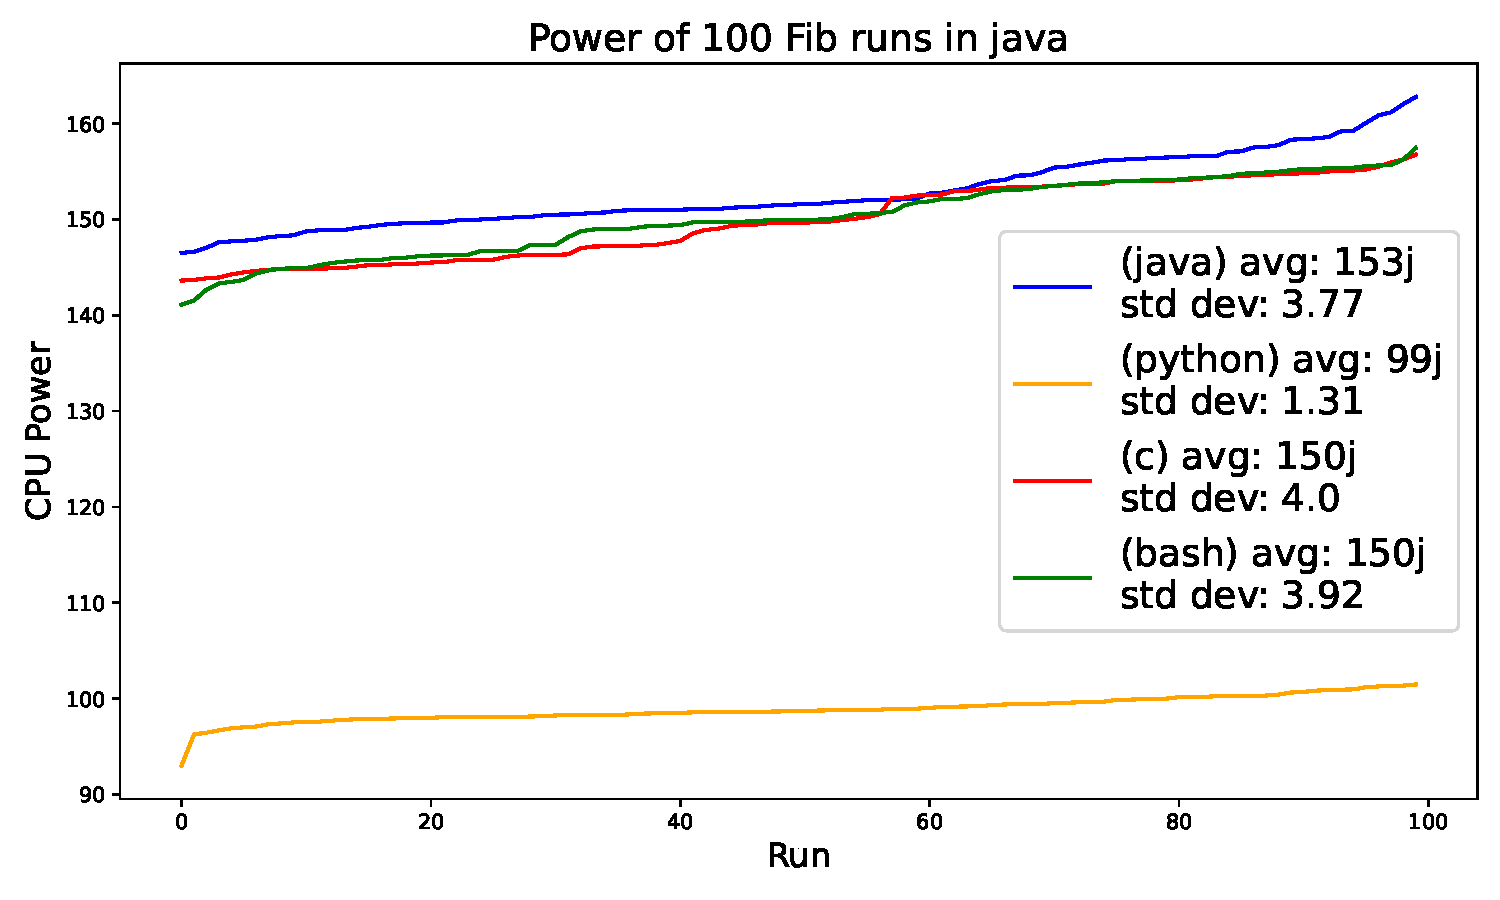
\includegraphics[width = 0.5 \textwidth]{figures/4_orchestrators_comparison.pdf}
%  \caption{orchestrators comparison}
%  \label{fig:4_orchs_comparison}
%\end{figure}